\documentclass[11pt, english, letterpaper]{article}
\usepackage[colorlinks=true, linkcolor=blue]{hyperref}
\usepackage[english]{babel}
\usepackage[utf8]{inputenc}
\usepackage[svgnames]{xcolor}
\usepackage[nomessages]{fp}
\usepackage{graphicx}
\usepackage{amsmath}
\usepackage{amsfonts}
\usepackage{fullpage}
\usepackage{appendix}
\usepackage{float}
\usepackage{listings}
\usepackage{afterpage}
\usepackage{here}
\usepackage{color}
\usepackage{ragged2e}
\usepackage[justification=centering]{caption}
\usepackage{indentfirst}
\usepackage{listings}
\usepackage{color}
\usepackage{subfig}
\usepackage[normalem]{ulem}
\useunder{\uline}{\ul}{}
\usepackage{longtable}
\usepackage{booktabs}
%----------------------------------------------------%

\pagestyle{plain}
\selectlanguage{english}
\setcounter{tocdepth}{2}

\definecolor{dkgreen}{rgb}{0,0.6,0}
\definecolor{gray}{rgb}{0.5,0.5,0.5}
\definecolor{mauve}{rgb}{0.58,0,0.82}

%----------------------------------------------------%

%% 
%% AMPL definition (c) 2007 Mirko Maischberger 
%% 

\lstdefinelanguage{AMPL}{ 
alsoletter={.},
morekeywords={Current,IN,INOUT,Infinity,Initial,LOCAL,OUT,all,binary,by,check,complements,contains,default,dimen,div,else,environ,exists,forall,if,in,integer,less,logical,max,min,option,setof,shell_exitcode,slve_exitcode,solve_message,solve_result,solve_result_num,suffix,sum,symbolic,table,then,union,until,while,within,from,to,obj,cross,diff,symdiff,inter,and,not,or,prod,product},%keywords
morekeywords=[2]{abs,acos,acosh,alias,asin,asinh,atan,atan2,atanh,ceil,ctime,cos,exp,floor,log,log10,max,min,precision,round,sin,sinh,sqrt,tan,tanh,time,trunc,Beta,Cauchy,Exponential,Gamma,Irand224,Normal,Normal101,Poisson,Uniform,Uniform01,num,num0,ichar,char,length,substr,sprintf,match,sub,gsub,card,next,nextw,prev,prevw,first,last,member,ord,ord0,arity,indexarity,interval,integer,ordered,circular,coeff,cover},%functions
morekeywords=[3]{set,param,var,arc,minimize,maximize,subject to,% 
node,subjto,s.t.},%declarations 
morekeywords=[4]{call,cd,check,close,commands,data,delete,display,drop,end,environ,exit,expand,fix,include,let,load,model,objective,option,print,printf,problem,purge,quit,read,readtable,redeclare,reload,remove,reset,restore,shell,show,solexpand,solution,solve,update,unfix,unload,write,write table,xref},%commands 
sensitive=true,% 
morecomment=[s]{/}{/},% 
morecomment=[l]\#,% 
morestring=[d]",% 
morestring=[d]'% 
}[keywords,comments,strings]% 

\lstset{frame=tb,
language=AMPL,
aboveskip=3mm,
belowskip=3mm,
showstringspaces=false,
columns=flexible,
numbers=none,
keywordstyle=\color{blue},
numberstyle=\tiny\color{gray},
commentstyle=\color{dkgreen},
stringstyle=\color{mauve},
breaklines=true,
breakatwhitespace=true,
tabsize=3
}

%----------------------------------------------------%

%\textheight=21cm
%\textwidth=17cm
%\topmargin=-1cm
%\oddsidemargin=0cm
%\parindent=0mm
%\pagestyle{plain}

\global\let\date\relax
\newcounter{unomenos}
\setcounter{unomenos}{\number\year}
\addtocounter{unomenos}{-1}
\stepcounter{unomenos}
\gdef\@date{ Course \arabic{unomenos}/ 2019}

%----------------------------------------------------%

\newcommand{\CC}{C\nolinebreak\hspace{-.05em}\raisebox{.4ex}{\tiny\bf +}\nolinebreak\hspace{-.10em}\raisebox{.4ex}{\tiny\bf +}}
\def\CC{{C\nolinebreak[4]\hspace{-.05em}\raisebox{.4ex}{\tiny\bf ++}}}

\newcommand{\I}{\mathcal{I}}
\newcommand{\J}{\mathcal{J}}
\newcommand{\SI}{\sum_{i \in I}}
\newcommand{\SJ}{\sum_{j \in J}}
\newcommand{\SK}{\sum_{k \in K}}
\newcommand{\SIJ}{\sum_{(i, j) \in I \times J}}
%\newcommand{\SIJ}{\sum_{\substack{i \in I \\ j \in J}}}
\newcommand{\SIK}{\sum_{(i, k) \in I \times K}}
\newcommand{\SJK}{\sum_{(j, k) \in J \times K}}
\newcommand{\SIJK}{\sum_{(i, j, k) \in I \times J \times K}}
%\newcommand{\SIJK}{\sum_{\substack{i \in I \\ j \in J \\ k \in K}}}

\newcommand{\valuestable}[9]{
Economy & #1 & #2 & #3 & \FPeval{\result}{clip((#1)+(#2)+(#3))} \result \\
Basic & #4 & #5 & #6 & \FPeval{\result}{clip((#4)+(#5)+(#6))} \result \\
Handcrafted & #7 & #8 & #9 & \FPeval{\result}{clip((#7)+(#8)+(#9))} \result \\
\hline
Total & \FPeval{\result}{clip((#1)+(#4)+(#7))} \result & \FPeval{\result}{clip((#2)+(#5)+(#8))} \result & \FPeval{\result}{clip((#3)+(#6)+(#9))} \result & \FPeval{\result}{clip((#1)+(#2)+(#3)+(#4)+(#5)+(#6)+(#7)+(#8)+(#9))} \result
}

\newcommand{\percenttable}[9]{
Economy & #1\% & #2\% & #3\% & \FPeval{\result}{clip((#1)+(#2)+(#3))} \result\% \\
Basic & #4\% & #5\% & #6\% & \FPeval{\result}{clip((#4)+(#5)+(#6))} \result\% \\
Handcrafted & #7\% & #8\% & #9\% & \FPeval{\result}{clip((#7)+(#8)+(#9))} \result\% \\
\hline
Total & \FPeval{\result}{clip((#1)+(#4)+(#7))} \result\% & \FPeval{\result}{clip((#2)+(#5)+(#8))} \result\% & \FPeval{\result}{clip((#3)+(#6)+(#9))} \result\% & \FPeval{\result}{clip((#1)+(#2)+(#3)+(#4)+(#5)+(#6)+(#7)+(#8)+(#9))} \result\%
}

\newcommand{\completetable}[3]{
\begin{table}[H]
\begin{center}
\begin{tabular}{c|ccc|c}
#2 & Student & Standard & Executive & Total \\
\hline
#1
\end{tabular}
\caption{#3}
\end{center}
\end{table}
}

%----------------------------------------------------%

\begin{document}

\begin{titlepage}

\begin{center}
\begin{figure}[htb]
\begin{center}

\includegraphics[width=6cm]{ucbseal.png}
\end{center}
\end{figure}

\vspace*{0.5in}
\Large{COLLEGE OF ENGINEERING - Fall 2019}\\
\vspace*{0.15in}
\Large{INDUSTRIAL ENGINEERING AND OPERATIONS RESEARCH DEPARTMENT - DATA SCIENCE (INDENG242)} \\
\vspace*{0.8in}
\begin{Large}
COURSE PROJECT:\\
\end{Large}
\vspace*{0.2in}
\begin{huge}
\textbf{Machine Learning For The Prediction Of The Success Of Altcoins} \\
\end{huge}
\vspace*{0.4in}
\rule{80mm}{0.1mm}\\
\vspace*{0.1in}
\begin{Large}
Made by: \\
Johnson Kanjirathinkal, Philippe Ferreira De Sousa, \\
Alejandro Sanchez Molina, Arun Putcha\\
\end{Large}
\vspace*{0.3in}

\includegraphics[width=6cm]{FungInstitute-logo.png}
\end{center}
\end{titlepage}


\tableofcontents

\newpage

\section{Motivation}
%\begin{justify}
\justify
Altcoins are alternative cryptocurrencies launched after the success of bitcoin. While the success of altcoins primarily depends on a number of factors such as the tech use case, funding, community and competition, general volume movement surges after they get listed on a major exchange.

\begin{figure}[!h]
    \centering
    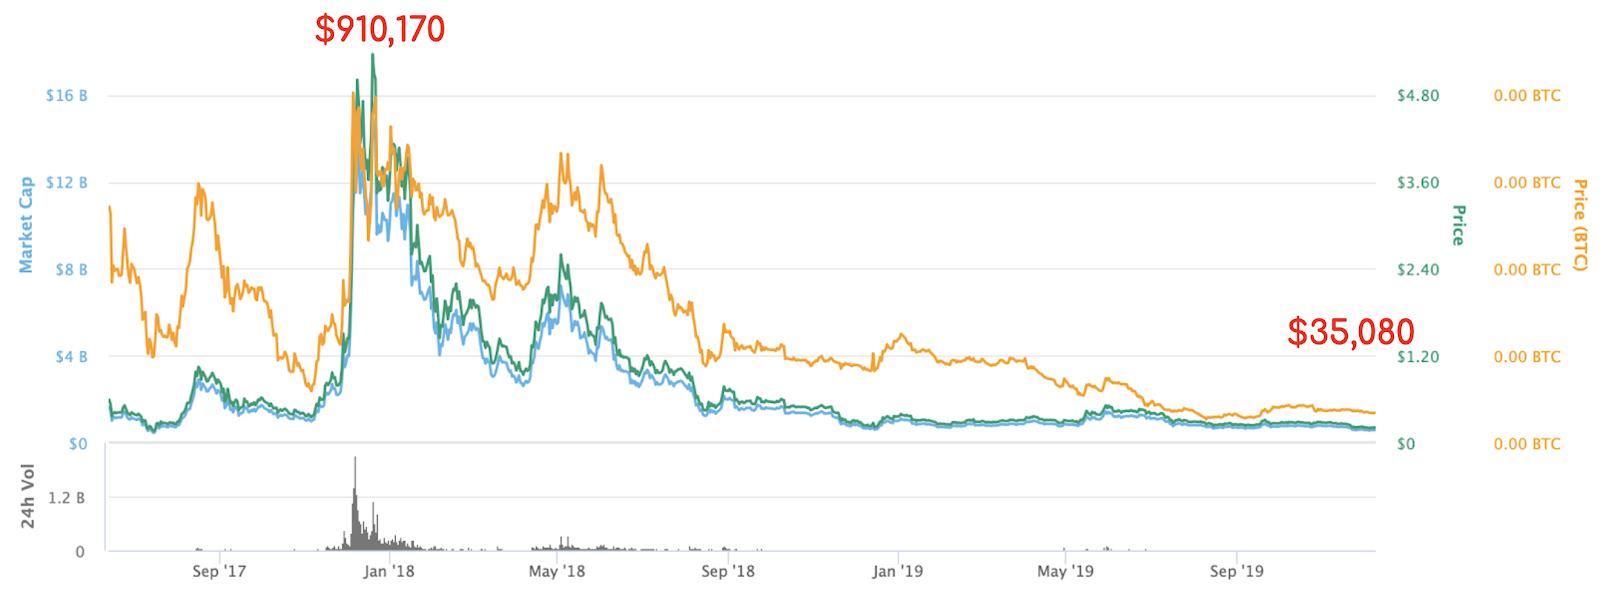
\includegraphics[width=\textwidth]{motivation_ICO.png}
    \caption{Value of \$100 of IOTA invested at the time of ICO}
\end{figure}

With the thousands of Initial Coin Offerings (ICOs), airdrops and obscure offerings that altcoins end up going through, we want to predict the likelihood of a particular set of  altcoins gaining in value over a period of time. For instance, Fig. 1 represents the value of 100\$ invested in IOTA at the time of ICO till date. The all time high was equivalent to \$910,170 and \$35,080 at the time of this report. Even if some of the portfolio of altcoins selected lose its value, the large growth rates of a small number would relate to profitability. This calculation has been considered for determination of portfolio value.

Identifying what makes an altcoin successful or unsuccessful has been hypothesized to be dependent on features not limited to the existence of a white paper, team credibility, Github activity, market cap etc. The data collection and modelling has been done to test these hypotheses.
%\ \begin{justify}
%\end{document}

\section{Data}

\begin{figure}[!h]
    \centering
    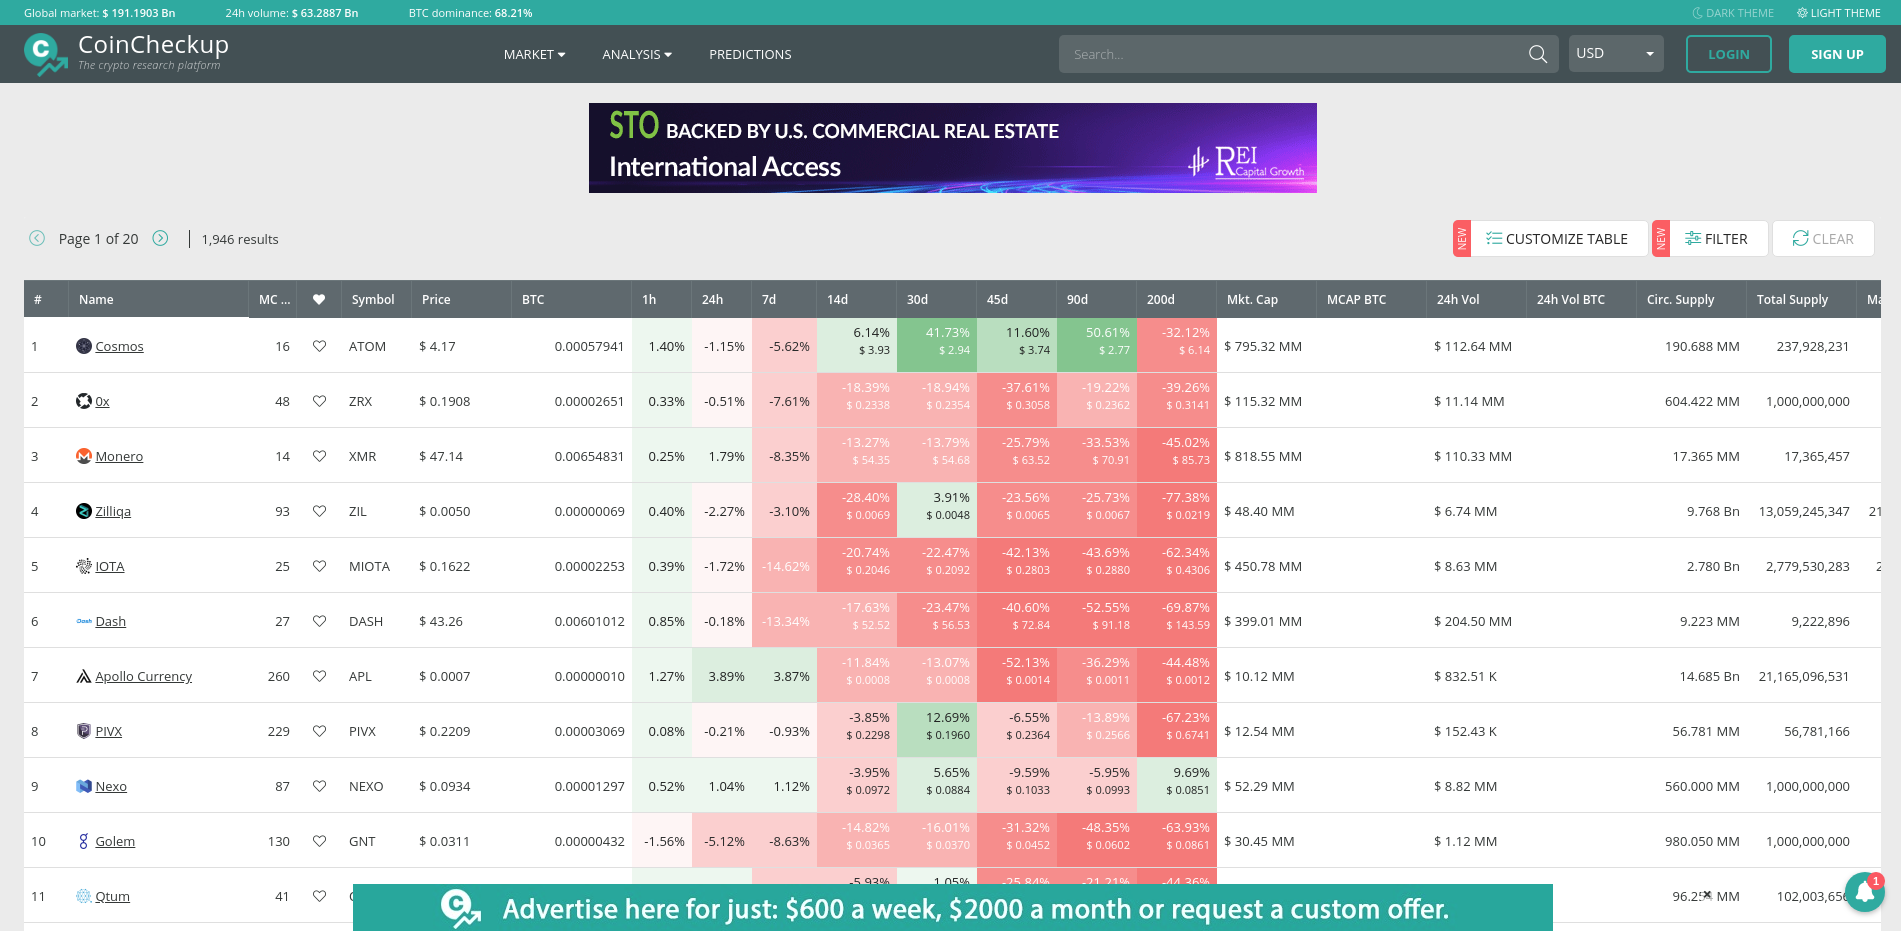
\includegraphics[width=\textwidth]{coincheckup.png}
    \caption{Fundamental analysis page of coincheckup.com}
\end{figure}

Historical altcoin data is not easily available publicly as a result of a variety of  coins constantly being added and removed. We determined that Coinmarketcap.com and Coincheckup.com provided sufficient resources for data collection pertaining to our problem statement. In order to evaluate the change in altcoin performance, we decided to consider a 10-month gap between our prediction estimation. All required data for this time frame was scrapped from the HTML from a historical snapshot from The Wayback Machine.  \par
The data from Feb 2019 had 1761 observations, while the data from Dec 2019 had 1916 observations. The count of common coins between these data sets was found to be 1460.  Fields that were considered to provide no value to the contribution of features was removed. Fields that had a large number of “NAs” were also dropped. As a consequence of altcoins purchases being done in exchange for BTC or ETH, all prices were converted to BTC, tied to the USD value of BTC on the day of the data snapshot. An assumption taken was that the market cap change would be of considerable importance. For cryptocurrencies, market cap is defined as the product of price and number of coins in circulation. However, it turns out the number of coins in circulation is modified or adjusted for a number of reasons. For instance, when it is discovered that some coins are lost forever (wallet seed is lost or destroyed) or the developers decide to “drop” privately held coins into circulation. As a result, this field was determined to be unreliable and removed from consideration for model building.  \par

\begin{figure}[!h]
    \centering
    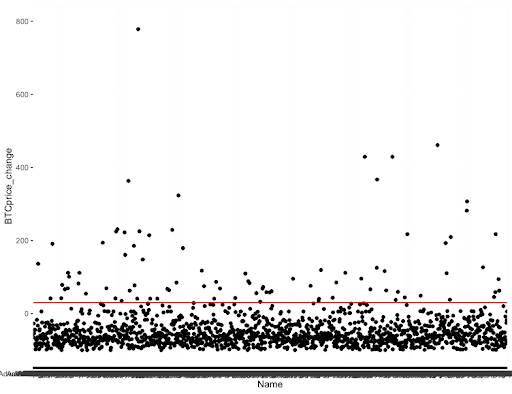
\includegraphics[width=0.8\textwidth]{data_ICO.png}
    \caption{Plot of BTC Price Change for all coins}
\end{figure}

For the creation of a test and training set, the percentage change in price was calculated for each coin based on the December and February data. This value was plotted and based on the number of coins, a growth of greater than 30\% was defined to be a successful outcome. A zoomed in plot of percentage change in price can be seen in Fig. 3. The red horizontal line marks the 30\% cut-off of the price change. This was used to create a column in the data frame to set a binary value for said outcome. 

Python files used to generate the dataset are attached in annex. We used \emph{parse.py}, \emph{parse\_ia.py} and \emph{parse\_fa.py} to parse the HTMl from 3 different pages of CoinCheckup.com, namely the fundamental analysis page (fa) and the investment analysis page (ia). It needs to be done for the version of the website in March and in December. Then we can merge all the data from March in \emph{merge\_fixed\_data.py}.

Then in \emph{add\_performance\_to\_merged\_data.py} we can read data from December and create 5 columns:
\begin{enumerate}
    \item label\_Price: price in December
    \item label\_growth\_rate\_Price: (label\_Price - Price)/Price
    \item label\_Mkt. Cap: Market Cap in December
    \item label\_growth\_rate\_Mkt. Cap: (label\_Mkt. Cap - Mkt. Cap)/Mkt. Cap
    \item label\_disappeared: whether a coin is listed in March but not in December
\end{enumerate}

\section{Dead coin prediction}

\subsection{Logistic regression}

The list of coins on Coincheckup.com is different between 10 months ago and now. Some have been added (new coins) and others have been removed. We label the removed coins as dead coins and the remaining coins as still alive. We want to predict the death of a coin over those 10 months based on the data that we had in March. As a result, we created a column "label\_disappeared" in the March dataset to tell whether the coin is dead or not. We split the dataset in 70\% training and 30\% testing (with fair distribution of dead coins in both parts).

\begin{table}[!h]
    \begin{center}
        \begin{tabular}{c|cc}
        \#    & Alive & Dead \\
              \hline
        Train & 1025  & 208  \\
        Test  & 439   & 89  
        \end{tabular}
    \end{center}
\end{table}

We begin with a logistic regression on the features which are numeric and have a very low rate of NAs. We check that our VIF is correct. Then we reduce the range of features to the relevant ones and make a final logistic model, that we compare to the baseline
We do a logistic regression with an arbitrary threshold $p=0.2$ and with an AIC of 1015.9 we get:

$$\hat{Y}_{dead} = sigmoid(-0.004 X_{X45d} - 0.032 X_{Social})$$
with $sigmoid: x \rightarrow \dfrac{1}{1+e^{-x}}$.
See appendix for feature descriptions.

We can make predictions on the test set and compare with the result 10 months later. The proportion of dead coins is around 20\% and when we predict that if a coin is dead, it is true more or less half of the time, so the model is not too bad!

\begin{center}
    \begin{tabular}{c|cc}
    Real\ Pred    & Alive & Dead \\
          \hline
    Alive & 320  & 117  \\
    Dead  & 37   & 52  
    \end{tabular} \quad \quad
    \begin{tabular}{c|ccc}
    Model & Accuracy & TPR & FPR \\
          \hline
    Baseline  & 83.1\%   & 0 & 0\\
    Logistic reg. & 70.5\%  & 58.4\% & 26.8\%  
    \end{tabular}
\end{center}

\begin{figure}[!h]
    \centering
    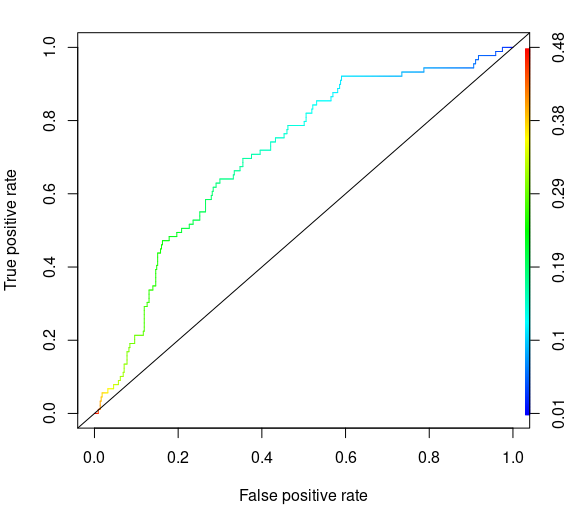
\includegraphics[width=0.5\textwidth]{ROC.png}
    \caption{ROC of the logistic regression (dead coin prediction)}
\end{figure}

\subsection{Random forest}

We began checking the number of NAs in each column to select the features. We choose: $X_{X24h}$, $X_{X14d}$, $X_{X45d}$, $X_{Social}$, $X_{Mkt. Cap}$, $X_{Age. mo.}$ and $X_{Business}$.
Then we try a random forest with cross-validation. We try a cross-validation measured with Accuracy and then F1-score as Accuracy is less relevant for unbalanced data.

\begin{figure}[!h]
    \centering
    \subfloat[Accuracy]{{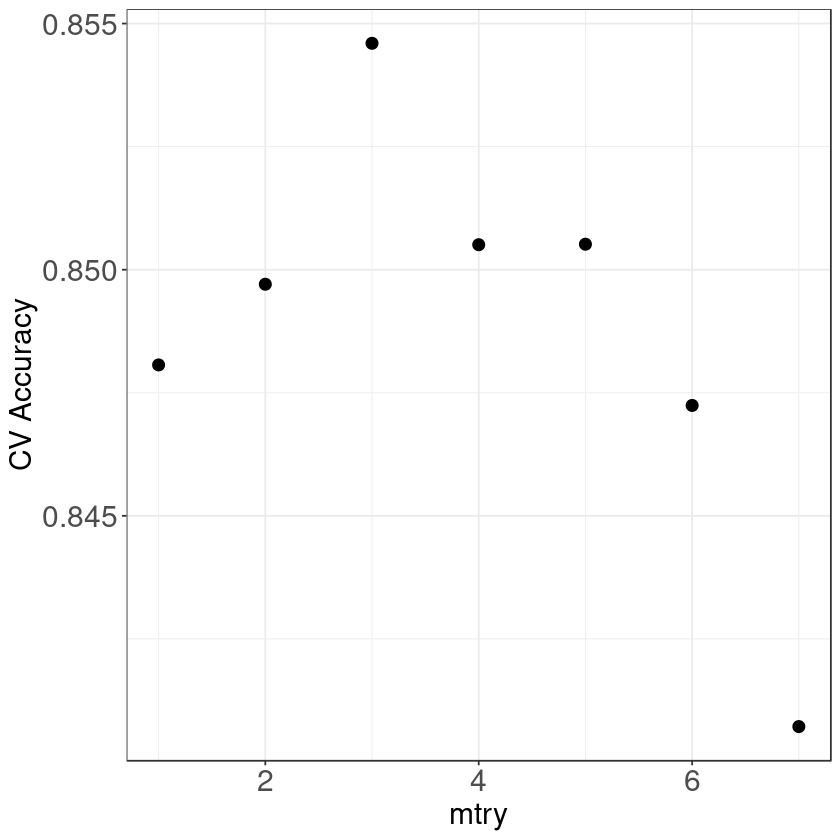
\includegraphics[width=7cm]{CV_acc_RF.png} }}%
    \qquad
    \subfloat[F1-score]{{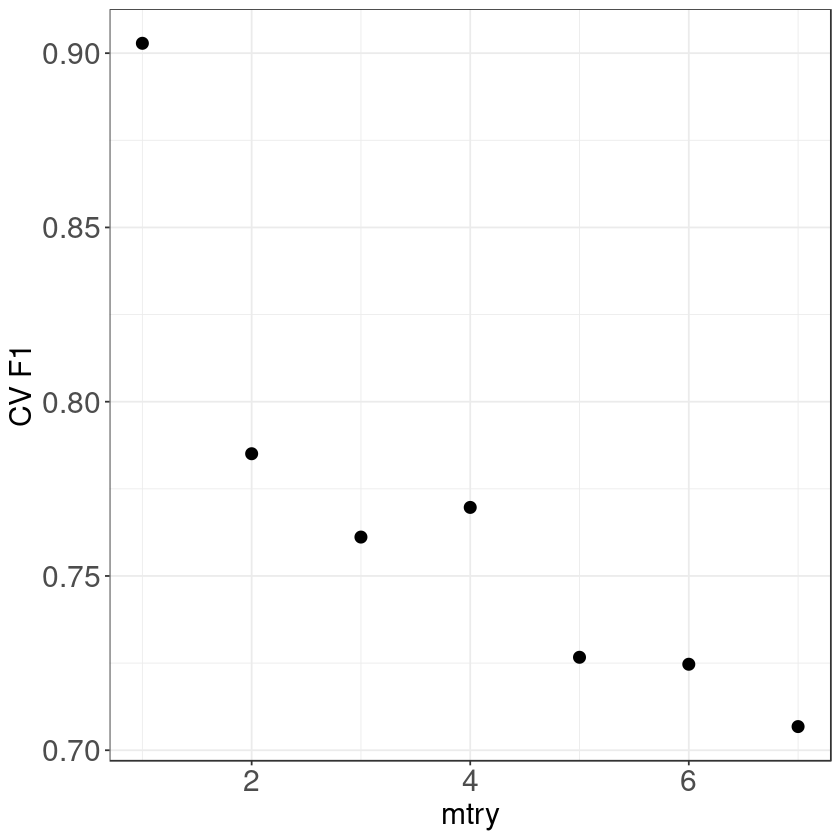
\includegraphics[width=7cm]{CV_F1_RF.png} }}%
    \caption{Cross validation of the random forest (dead coin prediction)}%
    \label{CV_RF}%
\end{figure}

Based on the results of figure \ref{CV_RF}, an mtry of 3 looks good. We can try sampling stratification to handle the imbalance of the data.

\begin{center}
    \begin{tabular}{c|cc}
    Real\ Pred    & Alive & Dead \\
          \hline
    Alive & 427  & 10  \\
    Dead  & 70   & 19  
    \end{tabular} \quad \quad
    \begin{tabular}{c|ccc}
    Model & Accuracy & TPR & FPR \\
          \hline
    Baseline  & 83.1\%   & 0 & 0\\
    Logistic reg. & 70.5\%  & 58.4\% & 26.8\%\\
    Random forest & 84.47\% & 21.35\% & 2.29\%
    \end{tabular}
\end{center}

\subsection{Gradient Boosting}

Finally we can try a gradient boosting method with cross-validation.

\begin{figure}[!h]
    \centering
    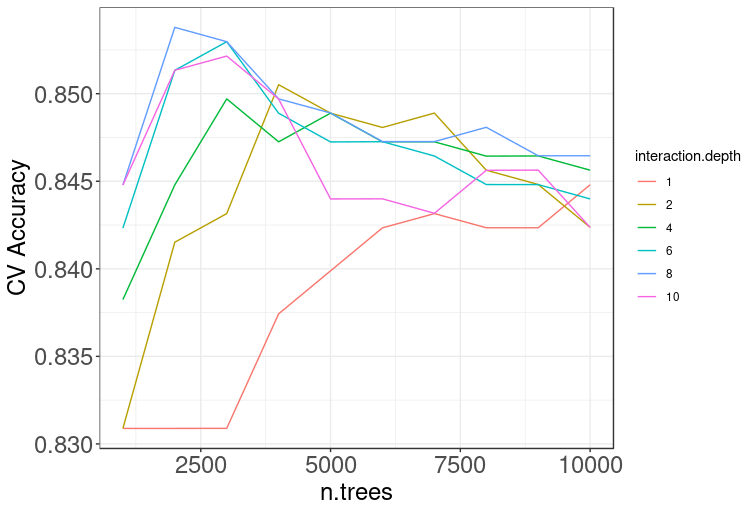
\includegraphics[width=0.8\textwidth]{CV_acc_boosting.png}
    \caption{Cross validation of the gradient boosting (dead coin prediction)}
    \label{CV_boosting}
\end{figure}

\begin{center}
    \begin{tabular}{c|cc}
    Real\ Pred    & Alive & Dead \\
          \hline
    Alive & 221  & 218  \\
    Dead  & 70   & 19  
    \end{tabular} \quad \quad
    \begin{tabular}{c|ccc}
    Model & Accuracy & TPR & FPR \\
          \hline
    Baseline  & 83.1\%   & 0 & 0\\
    Logistic reg. & 70.5\%  & 58.4\% & 26.8\%\\
    Random forest & 84.47\% & 21.35\% & 2.29\%\\
    Gradient boosting & 45.45\% & 21.35\% & 49.66\%
    \end{tabular}
\end{center}

Based on results from figure \ref{CV_boosting}, we choose n.trees = 2000, interaction.depth = 8.

\subsection{Conclusion}

Our random forest reaches the best accuracy, beating the baseline, while having a positive TPR and a low FPR.

Our gradient boosting model is very bad while the logistic regression threshold has been chosen to get the highest TPR, but it is at the expense of the accuracy and FPR.

\section{Portfolio determination based on naive growth rates}

Now let's tackle serious matters, we want to make money! To do that we need to establish a portfolio of assets. For now we assume that there is no opportunity cost for each asset to be in the portfolio. In practice there are fees to enter a position for each coin.

We want to naively predict $Y = label\growth\_rate\_Price = \dfrac{p_T-p_0}{p_0}$ over a period $T$ of 10 months.
After trying a linear regression on a lot of features, we stumble upon a multi-colinearity problem. So we remove the guilty features and then keep the few significant features:
$$Y = -2.53 \times 10^{-3} X_{Circ. Supply} + 9.58 \times 10^{-12} X_{Total. Supply} + \epsilon$$

\begin{center}
    \begin{tabular}{c|ccc}
    Model & MSE & MAE & OSR^2 \\
          \hline
    Baseline  & N/A   & N/A & N/A\\
    Linear reg. & 547.6 & 1.94 & -166.77
    \end{tabular}
\end{center}

It looks bad. We can compare it to the baseline (predicting negative all the time). We assume that we invest the same amount of money in each coin (ignoring fees) if we follow the baseline while we invest sizes $s_i = \dfrac{Y_i}{p_{0,i}}$ if we follow our regression strategy.
We can thus compute the result growth rate of both portfolios:
\begin{enumerate}
    \item Linear regression: $R = \dfrac{\sum_{i=1}^N s_i p_T^i - \sum_{i=1}^N s_i p_0^i}{ \sum_{i=1}^N s_i p_0^i} = \dfrac{\sum_{i=1}^N Y_i r_i}{\sum_{i=1}^N Y_i} = 0.142$
    \item Baseline: $R_b = \dfrac{\sum_{i=1}^N r_i}{N} = -0.342$
\end{enumerate}

Surprisingly we still beat the baseline on the test set and even earn money. We are lucky.

\section{Portfolio determination in a log normal stock model}

\subsection{Linear regression}

We often assume that the price of a stock follows a log-normal distribution, that is to say that for $S_t$ the price of an asset at time $t$, $log(S_t) \sim \mathcal{N}(\mu, \sigma^2)$. Let's $B_t$ be a standard Brownian motion ($\forall s<t, B_t - B_s \sim \mathcal{N}(0, t-s)$). We can write $S_t = S_0 e^{\mu t + \sigma B_t}$.
Then for a time $T > 0$ being our 10 months, $Y^{log} = log(S_T) - log(S_0) = \mu T + \sigma B_T$
where $B_T \sim \mathcal{N}(0, T)$.

Thus performing a linear regression $\forall 1 \leq i \leq n, Y^{log}_i = \beta_0 + \sum_{j=1}^p \beta_j X_{ij} + \epsilon_i$, we can try, assuming our parameters constant, to estimate $\mu = \dfrac{1}{T} (\beta_0 + \sum_{j=1}^p \beta_j X_{ij})$. However estimating $\sigma$ from $\epsilon$ would require us to assume that each coin has the same constant volatility which is too strong.

We need to do a new split of the data.
We come across a big multi-colinearity issue which forces us to remove some features. Making particular choices we find:

$$\hat{Y^{log}} = \mu T = -1.06 -0.00169 X_{X7d} -0.00033 X_{Market Cap} + 0.00412 X_{Age} + \epsilon$$

\begin{center}
    \begin{tabular}{c|cccc}
    Model & MSE & MAE & $OSR^2$ & R\\
          \hline
    Baseline & 1.35 & 0.774 & 0 & 0.413\\
    Linear reg. & 1.332  & 0.766 & 0.0152 & 0.50\\
    \end{tabular}
\end{center}

We can create a portfolio with sizes $s_i = exp(\hat{Y^{log}}_i)$.
Then our return is 

$R_{log} = \dfrac{\sum_{i=1}^N s_i p_T^i - \sum_{i=1}^N s_i p_0^i}{ \sum_{i=1}^N s_i p_0^i} = \dfrac{\sum_{i=1}^N s_i r_i}{\sum_{i=1}^N s_i} = 0.500$ against $R_b = \dfrac{\sum_{i=1}^N r_i}{N} = 0.413$ for the baseline.

Much better already! We see that filtering out coins where information is missing, our portfolio behaves already better! That's because trustworthy coins get all their information filled.

\subsection{Random forest}

We take the features from the 2 previous models and we try it out on a random forest.

\begin{figure}[!h]
    \centering
    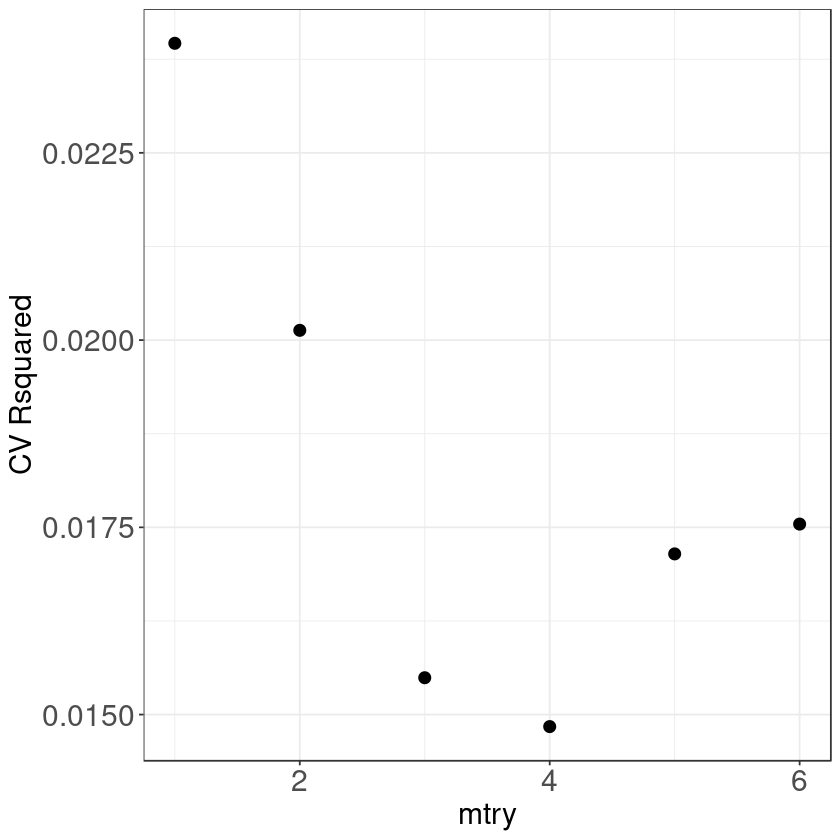
\includegraphics[width=0.5\textwidth]{CV_R2_RF}
    \caption{Cross validation of the random forest (log-normal model)}
\end{figure}

The best value is 1 for mtry.

\begin{center}
    \begin{tabular}{c|cccc}
    Model & MSE & MAE & $OSR^2$ & R\\
          \hline
    Baseline & 1.35 & 0.774 & 0 & 0.413\\
    Linear reg. & 1.332  & 0.766 & 0.0152 & 0.50\\
    Random forest & 1.343 & 0.768 & 0.005 & 0.318
    \end{tabular}
\end{center}

Unfortunately this model does not beat the baseline in term of financial gain.

\subsection{Gradient boosting}

We use the same features as for the random forest. After cross-validation (figure \ref{Boosting}, we conclude that the best parameters are the biggest ones.

\begin{figure}[!h]
    \centering
    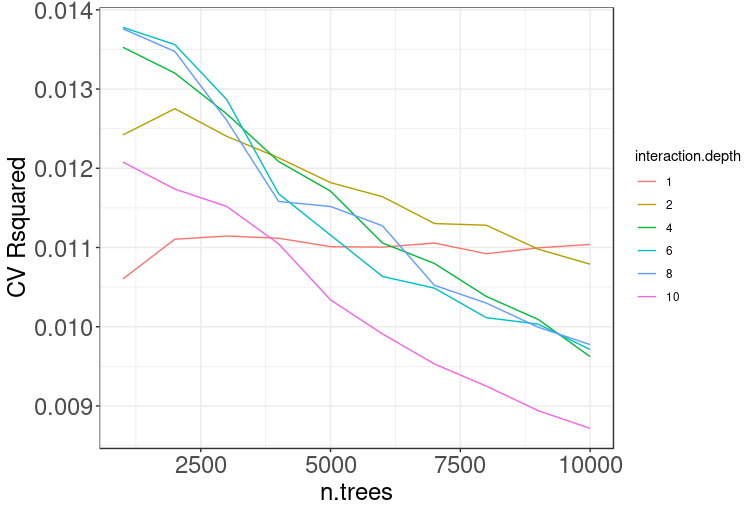
\includegraphics[width=0.5\textwidth]{CV_R2_boosting.png}
    \caption{Cross validation of the gradient boosting (log-normal model)}
    \label{Boosting}
\end{figure}

\begin{center}
    \begin{tabular}{c|cccc}
    Model & MSE & MAE & $OSR^2$ & R\\
          \hline
    Baseline & 1.35 & 0.774 & 0 & 0.413\\
    Linear reg. & 1.332  & 0.766 & 0.0152 & 0.50\\
    Random forest & 1.343 & 0.768 & 0.005 & 0.318\\
    Gradient boosting & 1.418 & 0.785 & -0.050 & 0.290
    \end{tabular}
\end{center}

This is also very bad compared to the baseline in term of porfolio return $R$.

\subsection{Conclusion}

The linear regression stays the best fit on the test set. The other model seem to overfit the data. Complicated models on low quality data makes bad results.

\section{Portfolio determination in real-world}

In reality there is an opportunity cost in choosing more coins in a portfolio. This cost comes form the fees to enter and exit the position: buy and sell fees plus withdraw fee (blockchain mining reward).
Using the model from previous section. If we choose the coin with the best predicted $\mu$ according to the linear regression, we get a growth rate $r = 2.067$ for CannabisCoin, which outperforms $R_{log}$.

The top 5 includes: CannabisCoin, GlobalBoost-Y, Quebecoin, SolarCoin, Curecoin.


\newpage

\section{Appendix}

\subsection{Column Definitions}


% Please add the following required packages to your document preamble:
% \usepackage[normalem]{ulem}
% \useunder{\uline}{\ul}{}
% \usepackage{longtable}
% Note: It may be necessary to compile the document several times to get a multi-page table to line up properly

\begin{longtable}{|p{5cm}|p{10cm}|}
\hline
\textbf{Column Name}   & \textbf{Description}                                                                                                                            \\ \hline
\endfirsthead
\endhead
MC..\_past             & Position of the coin the time of snapshot                                                                                                       \\ \hline
Symbol\_past           & Trading symbol for each coin                                                                                                                    \\ \hline
Price\_past            & Price in USD at the time of snapshot                                                                                                            \\ \hline
BTC\_past              & Price in BTC at the time of snapshot                                                                                                            \\ \hline
X30d\_past             & Percentage change in price over 30 days                                                                                                         \\ \hline
X45d\_past             & Percentage change in price over 45 days                                                                                                         \\ \hline
X90d\_past             & Percentage change in price over 90 days                                                                                                         \\ \hline
X200d\_past            & Percentage change in price over 200 days                                                                                                        \\ \hline
Mkt..Cap\_past         & Market Cap in USD                                                                                                                               \\ \hline
MCAP.BTC\_past         & Market Cap in BTC                                                                                                                               \\ \hline
Circ..Supply\_past     & No of circulating coins in supply                                                                                                               \\ \hline
Total.Supply\_past     & Total supply of coins                                                                                                                           \\ \hline
Max..Supply\_past      & Maximum supply of coins possible                                                                                                                \\ \hline
Team\_past             & Confidence value of the team based on past performance of leadership, developers etc, in percentage.                                            \\ \hline
Advisors\_past         & Confidence value of the  advisors, whether they have been successful historically and confirmed to be associated with said coin, in percentage. \\ \hline
Brand.Buzz\_past       & How large and active is the community as compared to the rest of the market, in percentage                                                      \\ \hline
Product\_past          & Is the coin an idea or a product at this stage, does it have a roadmap and available, confidence in percentage                                  \\ \hline
Coin\_past             & Confidence in ability to transact high volumes and availabilty, in percentage                                                                   \\ \hline
Social\_past           & Confidence in activity over social media, in percentage                                                                                         \\ \hline
Communication\_past    & Confidence of accessibility and activity over slack, telegram, email etc, in percentage                                                         \\ \hline
Business\_past         & Confidence in investors behind project, publishing of revenue reports etc, in percentage                                                        \\ \hline
GitHub\_past           & Confidence in activity on Github, in percentage                                                                                                 \\ \hline
Age..mo.\_past         & Age of the coins, in number of months                                                                                                           \\ \hline
Winning.months\_past   & No of successful months with positive growth over 12 months, in percentage                                                                      \\ \hline
Start.price\_past      & ICO start price                                                                                                                                 \\ \hline
CMGR....3mo\_past      & Compound Monthly Growth Rate trailing 3 months                                                                                                  \\ \hline
Cum..ROI\_past         & Cumulative ROI, the ROI in \% from start trading price till the current price                                                                   \\ \hline
Avg..volume\_past      & Average volume of coins traded                                                                                                                  \\ \hline
ATH\_past              & All time high of coin in USD                                                                                                                    \\ \hline
X..fm..ATH\_past       & Change in USD price from ATH, in percentage                                                                                                     \\ \hline
ATH..BTC.\_past        & All time high of coin in BTC                                                                                                                    \\ \hline
X..fm..ATH..BTC.\_past & Change in BTC price from ATH, in percentage                                                                                                     \\ \hline
Name                   & Name of the coin                                                                                                                                \\ \hline
Mkt.BTC\_c             & Market cap converstion from USD to BTC                                                                                                          \\ \hline
growth8mth             & Price change over month duration                                                                                                                \\ \hline
BTCprice\_change       & Percentage change in BTC compared to December                                                                                                   \\ \hline
BTCmcap\_change        & Market cap change of in BTC compared to December snapshot                                                                                       \\ \hline
success                & Binary value where 1 equals greater than 30\% increase in price                                                                                 \\ \hline
\end{longtable}

\newpage

\subsection{Python Code}

\hfill\break

\emph{parse.py}

\begin{lstlisting}
# URL = "https://web.archive.org/web/20190208144932/https://coincheckup.com/predictions"

import re
from bs4 import BeautifulSoup
import csv


datas = []
for tab_idx in range(1, 22):
    with open(f"html/20190208/predictions/Predictions Overview - CoinCheckup{tab_idx}.html") as file:
        soup = BeautifulSoup(file.read(), 'html.parser')

        cryptos = [link.string for link in soup.find_all('a') if link.get("href") and "coins" in link.get("href")]

        divs = [row for row in soup.find_all(attrs={"class": re.compile("ag-row ag-row-no-focus ag-row-\w* ag-row-level-0")}) if
                row.div is not None and row.div.span is None]
        data = [[cryptos[idx]] + [cell.string.strip("$ ").replace(',', '') for cell in div.children] for idx, div in enumerate(divs)]

        datas.append(data)


with open('coincheckup_10_months_predictions.csv', 'w', newline='') as csvfile:
    writer = csv.writer(csvfile, delimiter=',')
    writer.writerow([span.string for span in soup.find_all(role="columnheader")])
    for data in datas:
        for row in data:
            writer.writerow(row)

\end{lstlisting}


\newpage
\emph{parse\_fa.py}
\begin{lstlisting}
# URL = "https://web.archive.org/web/20190208144932/https://coincheckup.com/analysis"

import re
from bs4 import BeautifulSoup
import csv


def current():
    datas = []
    for tab_idx in range(1, 21):
        with open(f"html/20191205/fundamental_analysis/Analysis Overview - CoinCheckup{tab_idx}.html") as file:
            soup = BeautifulSoup(file.read(), 'html.parser')

            cryptos = [link.string for link in soup.find_all('a') if link.get("href") and "coins" in link.get("href")]

            divs = [row for row in soup.find_all(attrs={"class": re.compile("ag-row ag-row-no-focus ag-row-\w* ag-row-level-0")}) if
                    row.div is not None and row.contents[1].img is None]
            data = [[cryptos[idx]] + [div.contents[i].string if div.contents[i].div is None else div.contents[i].div.string for i in range(len(div.contents)-1) if i != 1] for idx, div in enumerate(divs)]
            for d in data:
                #print(d)
                for i in range(len(d)):
                    if d[i] is not None:  # Some 200d values are None
                        d[i] = d[i].strip("$% ")    # MM and K units should be handled here
            datas.append(data)


    with open('coincheckup_current_fa.csv', 'w', newline='') as csvfile:
        writer = csv.writer(csvfile, delimiter=',')
        ### WARNING: Problem with order in the column, FIXED HEADER
        header=['Name', 'MC #', 'Symbol', 'Price', 'BTC', '1h', '24h', '7d', '14d', '30d', '45d', '90d', '200d', 'Mkt. Cap', 'MCAP BTC', '24h Vol', '24h Vol BTC', 'Circ. Supply', 'Total Supply', 'Max. Supply', 'Team', 'Advisors', 'Brand/Buzz', 'Product', 'Coin', 'Social', 'Communication', 'Business', 'GitHub','GitHub', 'Avg. volume', 'Age (mo)', 'Winning months']
        #writer.writerow([span.string for span in soup.find_all(role="columnheader")[1:-1] if span.string is not None])
        writer.writerow(header)
        for data in datas:
            for row in data:
                writer.writerow(row)


def ten_months():
    datas = []
    for tab_idx in range(1, 19):
        with open(f"html/20190208/fundamental_analysis/Analysis Overview - CoinCheckup{tab_idx}.html") as file:
            soup = BeautifulSoup(file.read(), 'html.parser')

            cryptos = [link.string for link in soup.find_all('a') if link.get("href") and "coins" in link.get("href")]

            divs = [row for row in
                    soup.find_all(attrs={"class": re.compile("ag-row ag-row-no-focus ag-row-\w* ag-row-level-0")}) if
                    row.div is not None and row.contents[1].img is None]
            data = [
                [cryptos[idx]] + [div.contents[i].string if div.contents[i].div is None else div.contents[i].div.string
                                  for i in range(len(div.contents) - 2)] for idx, div in enumerate(divs)]

            for d in data:
                print(d)
                for i in range(len(d)):
                    ### WARNING: I modify this part because there is a column that is useless
                    if i <=2 :
                        if i == 2 :
                            continue
                        if d[i] is not None:  # Some 200d values are None
                            d[i] = d[i].strip("$% ")

                    else :
                        if d[i] is not None:  # Some 200d values are None
                            d[i-1] = d[i].strip("$% ")

            datas.append(data)

    with open('coincheckup_10_months_fa.csv', 'w', newline='') as csvfile:
        writer = csv.writer(csvfile, delimiter=',')

        ### WARNING: Problem with order in the column, FIXED HEADER
        header=['Name', 'MC #', 'Symbol', 'Price', 'BTC', '1h', '24h', '7d', '14d', '30d', '45d', '90d', '200d', 'Mkt. Cap', 'MCAP BTC', '24h Vol', '24h Vol BTC', 'Circ. Supply', 'Total Supply', 'Max. Supply', 'Team', 'Advisors', 'Brand/Buzz', 'Product', 'Coin', 'Social', 'Communication', 'Business', 'GitHub','GitHub', 'Avg. volume', 'Age (mo)', 'Winning months']
        #writer.writerow([span.string for span in soup.find_all(role="columnheader")[1:-1] if span.string is not None])
        writer.writerow(header)
        for data in datas:
            for row in data:
                writer.writerow(row)

current()
ten_months()
\end{lstlisting}


\newpage
\emph{parse\_ia.py}
\begin{lstlisting}
# URL = "https://web.archive.org/web/20190208144932/https://coincheckup.com/analysis"

import re
from bs4 import BeautifulSoup
import csv


def current():
    datas = []
    numeration=1
    for tab_idx in range(1, 25):
        with open(f"html/20191205/investment_analysis/Investment Overview - CoinCheckup{tab_idx}.html") as file:
            soup = BeautifulSoup(file.read(), 'html.parser')

            cryptos = [link.string for link in soup.find_all('a') if link.get("href") and "coins" in link.get("href")]

            divs = [row for row in soup.find_all(attrs={"class": re.compile("ag-row ag-row-no-focus ag-row-\w* ag-row-level-0")}) if
                    row.div is not None and row.contents[1].img is None]

            data = [[cryptos[idx]] + [cell.string.strip("$% ").replace(',', '') for cell in div.children] for idx, div in enumerate(divs)]

            datas.append(data)



    with open('coincheckup_current_ia.csv', 'w', newline='') as csvfile:
        writer = csv.writer(csvfile, delimiter=',')
        writer.writerow([span.string for span in soup.find_all(role="columnheader")[1:] if span.string is not None])
        for data in datas:
            for row in data:
                data.insert
                writer.writerow(row)


def ten_months():
    datas = []
    for tab_idx in range(1, 22):
        with open(f"html/20190208/investment_analysis/Investment Overview - CoinCheckup{tab_idx}.html") as file:
            soup = BeautifulSoup(file.read(), 'html.parser')

            cryptos = [link.string for link in soup.find_all('a') if link.get("href") and "coins" in link.get("href")]

            divs = [row for row in
                    soup.find_all(attrs={"class": re.compile("ag-row ag-row-no-focus ag-row-\w* ag-row-level-0")}) if
                    row.div is not None and row.contents[1].img is None]
            if len(cryptos) == 0:
                print("WARNING: File of idx {} is ignored because it contains no data".format(tab_idx))
                continue
            data = [[cryptos[idx]] + [cell.string.strip("$% ").replace(',', '') for cell in div.children] for idx, div in enumerate(divs)]

            datas.append(data)

    with open('coincheckup_10_months_ia.csv', 'w', newline='') as csvfile:
        writer = csv.writer(csvfile, delimiter=',')
        writer.writerow([span.string for span in soup.find_all(role="columnheader")[1:] if span.string is not None])
        for data in datas:
            for row in data:
                writer.writerow(row)
current()
ten_months()

\end{lstlisting}


\newpage
\emph{merge\_fixed\_data.py}
\begin{lstlisting}
import csv

num_fields = ['MC #', 'Price', 'BTC', '1h', '24h', '7d', '14d', '30d', '45d', '90d', '200d', 'Mkt. Cap', 'MCAP BTC', '24h Vol', '24h Vol BTC', 'Circ. Supply', 'Total Supply', 'Max. Supply', 'Team', 'Advisors', 'Brand/Buzz', 'Product', 'Coin', 'Social', 'Communication', 'Business', 'GitHub', 'Avg. volume', 'Age (mo)', 'Winning months']

with open("fixed_data/coincheckup_10_months_fa.csv", 'r', newline='') as old_fa, open("fixed_data/coincheckup_10_months_fa.csv", 'r', newline='') as old_ia:
    fa_reader = csv.DictReader(old_fa, delimiter=',')
    ia_reader = csv.DictReader(old_ia, delimiter=',')

    fields = set(fa_reader.fieldnames).union(set(ia_reader.fieldnames))
    #data = pd.DataFrame({field: [] for field in fields})
    data = {row["Name"]: row  for row in fa_reader}
    for row in ia_reader:
        for key, value in row.items():
            data[row["Name"]][key] = value

    for name, row in data.items():
        for field in num_fields:
            if row[field] in {'--', '---', '', 'N/A'}:
                row[field] = ''
            else:
                row[field] = float(row[field].strip("$% ").replace(',', '').replace(' ', '').replace('K', '000').replace('MM', '000000').replace('Bn', '000000000').replace('Tn', '000000000000'))

with open("merged_10months_data.csv", 'w', newline='') as output:
    writer = csv.DictWriter(output, delimiter=',', fieldnames=fields)
    writer.writeheader()
    for row in data.values():
        writer.writerow(row)
\end{lstlisting}


\newpage
\emph{add\_performance\_to\_merged\_data.py}

\begin{lstlisting}
import csv

with open("merged_10months_data.csv", 'r', newline='') as old, open("fixed_data/coincheckup_current_fa.csv", 'r', newline='') as label, open("dataset.csv", 'w', newline='') as output:
    reader_old = csv.DictReader(old, delimiter=',')
    reader_label = csv.DictReader(label, delimiter=',')

    data = {row["Name"]: row for row in reader_old}

    for row in reader_label:
        if row["Name"] not in data:
            continue

        data[row["Name"]]["Price"] = float(data[row["Name"]]["Price"])
        data[row["Name"]]["Mkt. Cap"] = float(data[row["Name"]]["Mkt. Cap"])# VeThor Token Market cap is always 0 the growth rate crashed
        data[row["Name"]]["label_Price"] = float(row["Price"].replace(',', ''))
        data[row["Name"]]["label_Mkt. Cap"] = float(row["Mkt. Cap"].replace(',', '').replace(' ', '').replace('K', '000').replace('MM', '000000').replace('Bn', '000000000').replace('Tn', '000000000000'))
        data[row["Name"]]["label_growth_rate_Price"] = (data[row["Name"]]["label_Price"] - data[row["Name"]]["Price"])/data[row["Name"]]["Price"]
        data[row["Name"]]["label_growth_rate_Mkt. Cap"] = 1 if data[row["Name"]]["Mkt. Cap"] == 0 else (data[row["Name"]]["label_Mkt. Cap"] - data[row["Name"]]["Mkt. Cap"])/data[row["Name"]]["Mkt. Cap"]  # VeThor Token's Market cap so the growth rate is 1
        data[row["Name"]]["label_disappeared"] = "FALSE"

    for row in data.values():
        if "label_Price" not in row:
            row["label_Price"] = row["label_Mkt. Cap"] = row["label_growth_rate_Price"] = row["label_growth_rate_Mkt. Cap"] = ""
            row["label_disappeared"] = "TRUE"


    writer = csv.DictWriter(output, delimiter=',', fieldnames=reader_label.fieldnames + ["label_Price", "label_Mkt. Cap", "label_growth_rate_Price", "label_growth_rate_Mkt. Cap", "label_disappeared"])
    writer.writeheader()
    for row in data.values():
        writer.writerow(row)
\end{lstlisting}

\subsection{Annotated R Code}

\end{document}



